\documentclass[review]{elsarticle}

%% Use the option review to obtain double line spacing
%% \documentclass[authoryear,preprint,review,12pt]{elsarticle}

%% Use the options 1p,twocolumn; 3p; 3p,twocolumn; 5p; or 5p,twocolumn
%% for a journal layout:
%% \documentclass[final,1p,times]{elsarticle}
%% \documentclass[final,1p,times,twocolumn]{elsarticle}
%% \documentclass[final,3p,times]{elsarticle}
%% \documentclass[final,3p,times,twocolumn]{elsarticle}
%% \documentclass[final,5p,times]{elsarticle}
%% \documentclass[final,5p,times,twocolumn]{elsarticle}

\usepackage{hyperref}
\usepackage{amsmath}
\usepackage{amssymb}
\usepackage{braket}
\usepackage{siunitx}
\usepackage[version=4]{mhchem}
\usepackage{tikz}
\usetikzlibrary{positioning}
\usetikzlibrary {arrows.meta} 
\usepackage{paralist}
\usepackage{todonotes}

%% The lineno packages adds line numbers. Start line numbering with
%% \begin{linenumbers}, end it with \end{linenumbers}. Or switch it on
%% for the whole article with \linenumbers.
%\usepackage{lineno}

\journal{Journal of Molecular Liquids}

\begin{document}
	
	\begin{frontmatter}
		
		%% Title, authors and addresses
		
		\title{Solvent effects on the prediction of redox potentials: application to nitroxides}
		
		\author[1]{Pierre Beaujean\corref{cor1}}
		
		\ead{pierre.beaujean@unamur.be}
		
		\cortext[cor1]{Corresponding author}
		
		\affiliation[1]{organization={Theoretical Chemistry Laboratory, Unit of Theoretical and Structural Physical Chemistry, Namur Institute of Structured Matter, University of Namur},%Department and Organization
			addressline={Rue de Bruxelles, 61}, 
			city={Namur},
			postcode={B-5000}, 
			country={Belgium}}
		
		\begin{abstract}
			This is an abstract
			
		\end{abstract}
		
		%%Graphical abstract
		\begin{graphicalabstract}
			%\includegraphics{grabs}
		\end{graphicalabstract}
		
		%%Research highlights
		\begin{highlights}
			\item Research highlight 1
			\item Research highlight 2
		\end{highlights}
		
		\begin{keyword}
			%% keywords here, in the form: keyword \sep keyword
			
			%% PACS codes here, in the form: \PACS code \sep code
			
			%% MSC codes here, in the form: \MSC code \sep code
			%% or \MSC[2008] code \sep code (2000 is the default)
			
		\end{keyword}
		
	\end{frontmatter}
	
	% \linenumbers
	
%% main text
\section{Introduction}

This is an introduction. It will contain:\begin{itemize}
	\item Batteries
	\item Nitroxides \cite{souleChemistryBiologyNitroxide2007}, Fig.~\ref{fig:states}
	\item Prediction of redox potential, and \textbf{the needs for a correct description of solvent-solute interactions}
	\item So: SMD, then Debye-Huckel, then CIP (or Matsui)
\end{itemize}

\begin{figure}[!h]
	\centering
	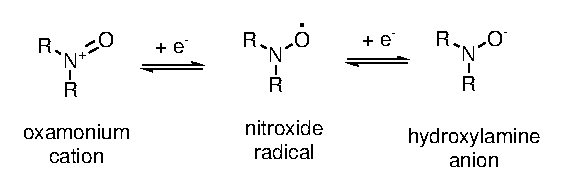
\includegraphics[width=.5\linewidth]{Figure1}
	\caption{Oxidized (left) and reduced (right) form of the the nitroxide radical (center).}
	\label{fig:states}
\end{figure}

\section{Theory}

In this section, different qualitative and quantitative models used in the analysis of the results are reviewed.

\subsection{Redox potentials in solution}

According to Ref.~\cite{marenichComputationalElectrochemistryPrediction2014}, the absolute reduction potential $E_{abs}^0$ (in \si{\volt}) of the half-reaction of reduction of $X^z$, $X^{z} + n_e\,e^- \rightarrow X^{z-n_e}$, reads: \begin{equation}
	E_{abs}^0(X^{z}|X^{z-n_e}) = -\frac{\Delta G_{r}^\star}{n_e\,F}, \text{ with } \Delta G_{r}^\star = G^\star(X^{z-n_e}) - G^\star(X^z), \label{eq:nernst}
\end{equation}
where $\Delta G_{r}^\star$ is the free Gibbs energy of the reduction reaction in solution, $F$ is the Faraday constant and $n_e$ the number of electrons involved in the reduction process. Last but not least, $G^\star(X^z)$ is the Gibbs free energy of $X^z$ in solution.  In the rest of this article, it is considered that $G^\star(e^-) = 0$.

From a phenomenological point of view, such energy is the sum of the one of the system in vacuum, plus the change in (free) energy resulting from its transfer to an electrolytic solution, \textit{i.e.}, $G^\star(X^z) = G^0(X^z)+ \Delta G_S^\star(X^z)$. The latter may be further decomposed using the thermodynamic cycle presented in Figure \ref{fig:th}. There are four steps: $\Delta G_d + \Delta G_s$ (discharge of a sphere in gas phase followed by charge in a dielectric) is a purely electrostatic processes, while $\Delta G_s$ is due, in most part, to non-electrostatic contributions (cavitation, vdW, etc). Finally, $\Delta G^\star_{DH}$ adds the effect of surrounding ions, and is therefore important to treat electrolytes \cite{silvaImprovingBornEquation2024}.

\begin{figure}[!h]
	\centering
	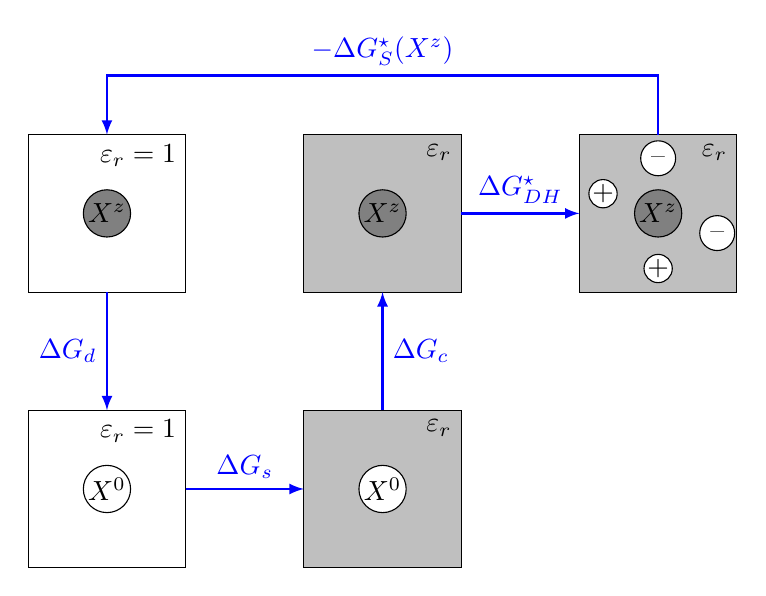
\begin{tikzpicture}
		\draw (-1,-1) rectangle +(2,2) node[anchor=north east]{$\varepsilon_r=1$};
		\draw[fill=gray] (0,0) circle (.3cm) node{$X^z$};
		
		
		\draw (-1,-4.5) rectangle +(2,2) node[anchor=north east]{$\varepsilon_r=1$};
		\draw (0,-3.5) circle (.3cm) node{$X^0$};
		
		
		\draw[fill=gray!50] (2.5,-4.5) rectangle +(2,2) node[anchor=north east]{$\varepsilon_r$};
		\draw[fill=white] (3.5,-3.5) circle (.3cm) node{$X^0$};
		
		
		\draw[fill=gray!50] (2.5,-1) rectangle +(2,2) node[anchor=north east]{$\varepsilon_r$};
		\draw[fill=gray] (3.5,0) circle (.3cm) node{$X^z$};
		
		
		\draw[fill=gray!50] (6,-1) rectangle +(2,2) node[anchor=north east]{$\varepsilon_r$};
		\draw[fill=gray] (7,0) circle (.3cm) node{$X^z$};
		\draw (2.8+3.5,-3.25+3.5) node[draw,fill=white,circle,inner sep=0]{+}
		(3.5+3.5,-2.8+3.5) node[draw,fill=white,circle,inner sep=.075cm]{--}
		(4.25+3.5,-3.75+3.5) node[draw,fill=white,circle,inner sep=.075cm]{--}
		(3.5+3.5,-4.2+3.5) node[draw,fill=white,circle,inner sep=0]{+};
		
		\draw[blue,thick,-latex] (0,-1) -- +(0,-1.5) node[midway,left]{$\Delta G_d$};
		\draw[blue,thick,-latex] (1,-3.5) -- +(1.5,0) node[midway,above]{$\Delta G_s$};
		\draw[blue,thick,-latex] (3.5,-2.5) -- +(0,1.5) node[midway,right]{$\Delta G_c$};
		\draw[blue,thick,-latex] (4.5,0) -- +(1.5,0) node[midway,above]{$\Delta G^\star_{DH}$};
		\draw[blue,thick,-latex] (7,1) -- ++(0,.75) -- node[midway,above]{$-\Delta G_S^\star(X^z)$} ++(-7,0) -- ++(0,-.75);
	\end{tikzpicture}
	\caption{Thermodynamic cycle to compute the energy of solvatation of an ion, $X^z$, in a electrolyte (solvent characterized by a $\varepsilon = \varepsilon_0\,\varepsilon_r$ dielectric constant and by a ``cloud'' of other ions). $\Delta G_d$ is the discharge of $X^z$ in gas phase, $\Delta G_s$ is the solvatation of $X$, $\Delta G_c$ is the charging of $X$ in $\varepsilon$, and $\Delta G^\star_{DH}$ is the addition of the other ions.}
	\label{fig:th}
\end{figure}


On the one hand, at the quantum chemistry (QC) level, the solvatation energy is generally treated implicitly, thanks to a self-consistent reaction field approach (SCRF) \cite{herbertDielectricContinuumMethods2021}: \begin{align}
	G^\star_{SCRF}(X) &= \Braket{\Psi|{\hat{H}+\frac{1}{2}\hat{R}}|\Psi} + G_{th}[\Psi] + G_{nonelst}(X) \nonumber\\
	&= E[\Psi] + G_{th}[\Psi] + \underbrace{G_{elst}[\Psi] + G_{nonelst}(X)}_{\Delta G^\star_{S,SCRF}(X)}, \label{eq:scrf}
\end{align}
where $\Psi$ is the wavefunction of $X$ (minimized under the application of $\hat R$, so not equal to the gas phase wavefunction), $\hat H$ is the electronic Hamiltonian, $\hat R$ is the reaction field operator (generally recognized to give rise to the electrostatic contribution to the solvation energy, $G_{elst}$), $G_{th}$ are the thermal contributions to the Gibbs free energy derived from thermostatistic analysis, and $G_{nonelst}$ is the non-electrostatic contributions (cavitation, dispersion, etc) to the solvation energy. Therefore, using the notation of Figure \ref{fig:th} (and assuming no change in the geometry of $X^z$), $ \Delta G^\star_{S,SCRF}(X^z) = \Delta G_d + \Delta G_s + \Delta G_{c}$.  

On the other hand, the Debye-Huckel (DH) theory provide another estimate of $\Delta G_{S}^\star$ \cite{bockrisModernElectrochemistryIonics1998}. Indeed, assuming that a ion $X^z$, bearing a charge $q = z\,e_0$ ($e_0$ is the elementary charge), can be approximated by a sphere of radius $a$ and that the ions in the solution are distributed in the solution according to Maxwell-Boltzmann statistics, one obtains the corresponding solvation energy as \cite{kontogeorgisDebyeHuckelTheoryIts2018,silvaDerivationsDebyeHuckel2022,silvaImprovingBornEquation2024}:\begin{align}
	\Delta G^\star_{S,DH}(X^z)
	&= \Delta G^\star_{born}(X^z) + \Delta G^\star_{DH}(X^z)\label{eq:adh}
\end{align}
where:
\begin{equation}
	\Delta G^\star_{Born}(X^z) =\frac{q^2}{8\pi\varepsilon_0\,a}\,\left[\frac{1}{\varepsilon_r}-1\right], \label{eq:born}\\
\end{equation}
and,
\begin{align}
	&\Delta G^\star_{DH}(X^z) = -\frac{q^2}{4\pi\varepsilon_0\varepsilon_r}\,\frac{\kappa}{(\kappa\,a)^3}\,\left[\ln(1+\kappa\,a)-\kappa\,a+\frac{1}{2}(\kappa\,a)^2\right],\label{eq:dh} \end{align}
in which $\kappa$ is the inverse of the Debye screening length, defined from:\begin{equation}
	\kappa^2 = \sum_i \frac{n_i\,q_i^2}{\varepsilon_0\varepsilon_r\,k_B\,T}, \label{eq:kappa2}
\end{equation}
where $n_i$ is the number density ($n_i = N_i / V = c_i\,\mathcal{N}_a$ where $\mathcal{N}_a$ is the Avogadro number and $c_i$ is the concentration in ion $i$) of ion of type $i$, $k_B$ is the Boltzmann constant, and $T$ is the temperature.  $\kappa$ is  proportional to the ionic strength of the solution, $I = \frac{1}{2}\sum_i c_i\,z_i^2$.  The Born part is generally dominant in solvatation energies predicted by this model (Fig.~S1).

In the limit of $\kappa\to 0$,  $\Delta G^\star_{DH} = 0$ and thus $\Delta G^\star_S \approx \Delta G^\star_{born} = \Delta G_d + \Delta G_c$.  Therefore, by combining Eqs.~\eqref{eq:scrf} and \eqref{eq:adh}, one defines:\begin{equation}
	G^\star(X^z) = G^\star_{SCRF}(X^z) + \Delta G^\star_{DH}(X^z), \label{eq:gtot}
\end{equation}
to be used in Eq.~\eqref{eq:nernst}. It should provide similar results to the approach developed by Cossi \emph{et al.} in Ref.~\citenum{cossiInitioStudyIonic1998}.

\subsection{Model for the impact of the substituent}

In first approximation, the electrostatic interaction between the substituent(s) and the charge formed upon oxidation or reduction affects the redox potential of nitroxides. In particular, assuming a non-charged substituent, charge-dipole interactions are stabilizing the oxiamonium ( $>$\ce{N+=O}) if the dipole is aligned with the charge, while this destabilize the hydroxylamine ( $>$\ce{N-O-}), both resulting in a decrease of the redox potential (Fig.~\ref{fig:dipole}). Within this framework, it is therefore expected that donor substituent have lower redox potential than acceptor.

\begin{figure}[!h]
	\centering
	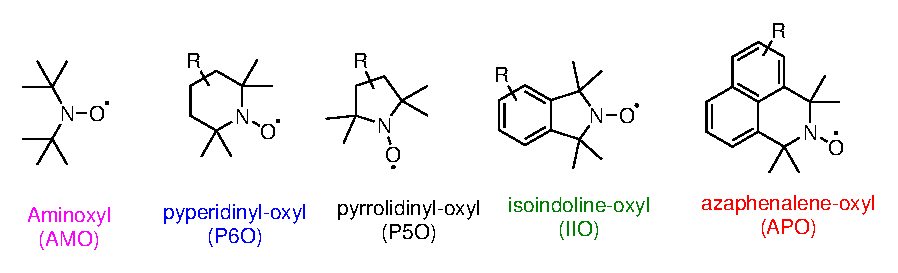
\includegraphics[width=.7\linewidth]{Figure2}
	\caption{Impact of the dipole orientation of the substituent on the redox potential when the dipole is oriented in  the positive $x$ direction (red) or not (blue). Adapted from Ref.~\citenum{zhangEffectHeteroatomFunctionality2018}.}
	\label{fig:dipole}
\end{figure}

In 2018, this model has been extended and applied by Zhang \textit{et al} \cite{zhangEffectHeteroatomFunctionality2018} to the oxidation potential. They further expanded the electrostatic interaction as  multipoles, truncated after third order, to include the large quadrupole moment of aromatic compounds:\begin{equation}
	U_q(r) = \frac{\mu_x}{r^2} + \frac{Q_{xx}}{r^3}, \label{eq:Er}
\end{equation}
assuming a non-charged substituent. The different quantities (dipole moment, $\mu_x$, and traceless quadrupole moment, $Q_{xx}$) are evaluated through a single point calculation on a simplified structure, using the geometry of the radical where the $>$\ce{N-O^.} moiety is substituted by \ce{CH_2}.  In this contribution, since the alignment of the dipole with the charge need to be accounted for, this geometry is oriented so that the $x$ axis pass through origin and the nitrogen, the origin being placed at the carbon bearing the substituent. $r$ is the origin-nitrogen distance. This definition for the origin is different from the original model, since  Zhang and co-workers did not consider multiple positions for a given substituent. 


\subsection{Impact of ion-pair formation on redox potentials}

At large concentration in electrolyte, one expect the formation of ions pairs in solution (insights are provided in the next subsection).  In this paper, the electrolyte is a pair, \ce{AC}, of counterions, where \ce{A-} and \ce{C+} are the cation and the ion, respectively. Furthermore, two state of complexation  are considered: \begin{inparaenum}[(i)]
	\item the pairs NA and NC between the oxidized (\ce{N+}) and reduced (\ce{N-}) state of nitroxide, with its corresponding counterion (\ce{A-} and  \ce{C+},  respectively (with a complexation constant $K_{x1}$) and then
	\item complexation with the \ce{AC} pair (with a complexation constant $K_{x2}$) , which is seen when concentration in electrolyte becomes large  \cite{wylieImprovedPerformanceAllOrganic2019a}.
\end{inparaenum}
The different equilibrium constants are defined in Fig.~\ref{fig:cip}.

\begin{figure}[!h]
	\centering
	\newcommand{\arrwy}[3]{
		\draw [transform canvas={yshift=0.3ex},arrows = {-Stealth[harpoon]}] (#1) -- (#2) node[midway,above]{#3};
		\draw [transform canvas={yshift=-0.3ex},arrows = {-Stealth[harpoon]}] (#2) -- (#1);
		}
		\newcommand{\arrwx}[3]{
		\draw [transform canvas={xshift=0.3ex},arrows = {-Stealth[harpoon]}] (#1) -- (#2) node[midway,left]{#3};
		\draw [transform canvas={xshift=-0.3ex},arrows = {-Stealth[harpoon]}] (#2) -- (#1);
		}
	\begin{tikzpicture}[node distance=2cm]
		\node (N1) {\ce{N+ + A- + C+ + 2e-}};
		\node[right=1cm of N1] (N1c) {\ce{NA + C+ + 2e-}};
		\arrwy{N1.east}{N1c.west}{$K_{01}$}
		\node[left=1cm of N1] (N1cc) {\ce{NAC+ + 2e-}};
		\arrwy{N1cc.east}{N1.west}{$K_{02}$}
		
		\node[below of = N1] (N2) {\ce{N^. + A+ + C- + e-}};
		\arrwx{N1.south}{N2.north}{$K_{1}$}
		\node[below of=N1cc] (N2cc) {\ce{NAC^. + e-}};
		\arrwy{N2cc.east}{N2.west}{$K_{12}$}
		
		\node[below of=N2] (N3) {\ce{N- + A- + C+}};
		\arrwx{N2.south}{N3.north}{$K_2$}
		\node[right= 2cm of N3] (N3c) {\ce{NC  + A-}};
		\arrwy{N3.east}{N3c.west}{$K_{21}$}
		\node[below of=N2cc] (N3cc) {\ce{NAC-}};
		\arrwy{N3cc.east}{N3.west}{$K_{22}$}
	\end{tikzpicture}
	\caption{Scheme illustrating the different possible reactions: \ce{N+} and \ce{N-} are the oxidized and reduced forms of a given nitroxide, \ce{N^.}, and \ce{C+} and \ce{A-} are the countercation and anion coming from electrolyte, respectively. Horizontal arrows are ion-pairing reactions (with the \ce{AC} pair in left, with a single counterion in right), while vertical arrows are electrochemical reactions.}
	\label{fig:cip}
\end{figure}

Following Mugisa and co-workers \cite{mugisaEffectIonparingKinetics2024}, a quantitative model is derived from Fig.~\ref{fig:cip}, owing that:  \begin{inparaenum}[(i)]
	\item the total concentration in redox active species is given by $c_{ox} = [\ce{N+}]+[\ce{NA}] + [\ce{NAC+}]$, $c_{rad} = [\ce{N^.}] + [\ce{NAC^.}]$ and $c_{red} =  [\ce{N-}]+[\ce{NC}] + [\ce{NAC-}]$, 
	\item given electroneutrality, $ [\ce{C+}] = [\ce{A-}] $,
	\item the electrolyte is in large amount with respect to redox active species, and thus $[X] = [\ce{C+}] = [\ce{A-}] $ is a constant ($[X]$ is the electrolyte concentration), and
	\item at the equilibrium of redox redaction, $c_{ox} = c_{rad}$ ($K_1$) and $c_{red} = c_{rad}$ ($K_2$).
\end{inparaenum}
Within these assumption, the following electrolyte concentration-dependent (formal) redox potentials are obtained:\begin{align}
	E^f_{abs}(\ce{N+|N^.}) &= E^0_ {abs}(\ce{N+|N^.})+\frac{RT}{F}\,\ln\left[\frac{1+K_{12}\,[X]^2}{1+K_{01}\,[X]+K_{02}\,[X]^2}\right],\\
	E^f_{abs}(\ce{N^.|N-}) &= E^0_ {abs}(\ce{N^.|N-})+\frac{RT}{F}\,\ln\left[\frac{1+K_{21}\,[X]+K_{22}\,[X]^2}{1+K_{12}\,[X]^2}\right],
\end{align}
in which $K_{ij}= e^{-\frac{\Delta G_{ij}^\star}{RT}}$, where $\Delta G_{ij}^\star$ is the free Gibbs energy change [computed with Eq.~\eqref{eq:gtot}] for a given complexation reaction.

An example is provided in Fig.~S2: while $K_{x1}$ dictates the behavior at low $[X]$, but the trend at large $[X]$ is given by $K_{12} / K_{02}$ (oxidation) and $K_{22} / K_{12}$ (reduction).

\subsection{Model for the ion-pair formation}

Insight in the formation of ion pairs ($K_{01}$ and $K_{21}$ in Fig.~\ref{fig:cip}) is provided by a simple model proposed by Lund et al. \cite{lundDielectricInterpretationSpecificity2010}. It is based on the balance between the solvatation of the individual charges [described by the Born model, Eq.~\eqref{eq:born}] and the formation of a dipole when the two charges are in interaction, leading to the famous Onsager model \cite{onsagerElectricMomentsMolecules1936,aubretUnderstandingLocalField2019}. From the thermodynamic cycle given in Fig.~\ref{fig:ionpair}, one derive the following expression:\begin{equation}
	\Delta G_{pair}^\star = \frac{1}{4\pi\varepsilon_0}\,\left\{\left[\frac{q_1^2}{2a_1}+\frac{q_2^2}{2a_2}\right]\,\left[1-\frac{1}{\varepsilon_r}\right]+\frac{q_1\,q_2\,|q_1-q_2|}{2\,\mu}-\frac{\varepsilon_r-1}{2\varepsilon_r+1}\,\frac{\mu^2}{a^3}\right\},
\end{equation}
where $a_1$, $a_2$ and $a=s_2\,( a_1^3+a_2^3)^{1/3}$ are the radii of the cavity corresponding to $q_1$, $q_2$, and the dipole, respectively, defined as $\mu = \frac{s_1}{2}\,|q_2-q_1|\,(a_1+a_2)$.  $s_1$ and $s_2$ are scaling factors, which accounts for the electrostatic attraction between the two charge forming the dipole ($s_1\leq 1$) and the fact that the cavity might not be spherical ($s_2\geq 1$).

\begin{figure}[!h]
	\centering
	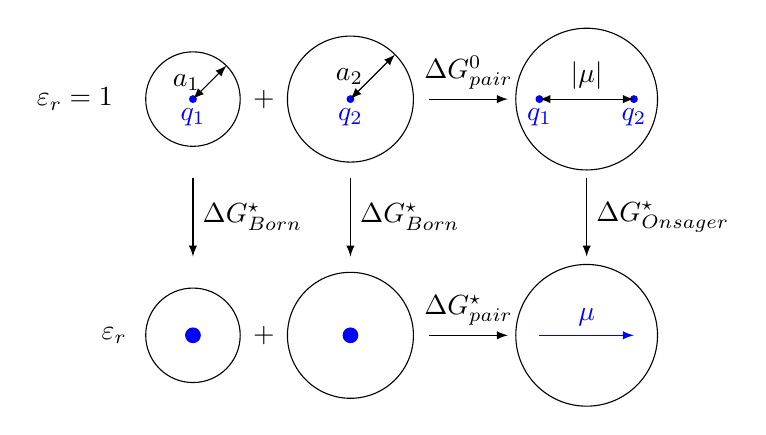
\begin{tikzpicture}
		\draw (-1.5,0) node{$\varepsilon_r=1$};
		\draw (-1,-3) node{$\varepsilon_r$};
		\draw (0,0) circle (.6cm);
		\fill[blue] (0,0) node[below]{$q_1$}  circle (.05cm);
		\draw[latex-latex] (0,0) -- (45:0.6) node[midway,left]{$a_1$};
		
		\draw (.9,0) node{+};
		
		\draw (2,0) circle (.8cm);
		\fill[blue] (2,0) node[below]{$q_2$}  circle (.05cm);
		\draw[latex-latex] (2,0) -- +(45:0.8) node[midway,left]{$a_2$};
		
		\draw[-latex] (3,0) -- +(1,0) node[midway,above]{$\Delta G^0_{pair}$};
		
		\draw (5,0) circle (.9cm);
		\fill[blue] (4.4,0) node[below]{$q_1$} circle (.05cm);
		\fill[blue] (5.6,0) node[below]{$q_2$}  circle (.05cm);
		\draw[latex-latex](4.4,0) -- (5.6,0) node[midway,above]{$|\mu|$};
		
		\draw[-latex] (0,-1) -- +(0,-1) node[midway,right]{$\Delta G^\star_{Born}$};
		\draw[-latex] (2,-1) -- +(0,-1) node[midway,right]{$\Delta G^\star_{Born}$};
		\draw[-latex] (5,-1) -- +(0,-1) node[midway,right]{$\Delta G^\star_{Onsager}$};
		
		\fill[blue] (0,-3) circle (.1cm);
		\draw (0,-3) circle (.6cm);
		
		\draw (.9,-3) node{+};
		
		\draw (2,-3) circle (.8cm);
		\fill[blue] (2,-3) circle (.1cm);	
		
		\draw[-latex] (3,-3) -- +(1,0) node[midway,above]{$\Delta G^\star_{pair}$};
		
		\draw (5,-3) circle (.9cm);
		\draw[-latex,blue](4.4,-3) -- (5.6,-3) node[midway,above]{$\mu$};
	\end{tikzpicture}
	\caption{Thermodynamic cycle for the formation of ion-pair, adapted from Ref.~\citenum{lundDielectricInterpretationSpecificity2010}.}
	\label{fig:ionpair}
\end{figure}

This qualitative model (Fig.~S3) shows that ion-pairing depends on: \begin{inparaenum}[(i)]
	\item the ratio, $\chi = a_1 / a_2$, with $\chi \sim 1$ leading to the lowest pair formation energy (which was already pointed out by Lund and co-workers), 
	\item the attraction between the charges ($s_1$), 
	\item the shape of the final cavity (pairing energy increases with $s_2$), and
	\item the dielectric constant $\varepsilon_r$.
\end{inparaenum}
While this latter parameter only has a minor influence (but the difference increases with $s_1$), the formation of a pair of ions is favored in less polar solvents, as expected.\todo{Le modele est intéréssant pour les liquides ioniques, soit dit en passant}

\section{Methodology}

In this contribution, the set of nitroxides considered by Hogsdon \textit{et al.} (compounds \textbf{1}-\textbf{54}) is considered, with a few extra compounds for completeness (\textbf{55}-\textbf{61}). All structures are provided in Fig.~\ref{fig:nitroxides}. The \ce{AC} pair formed by \ce{BF4^-} (\ce{A-}) and \ce{NMe4^+} (\ce{C+}) is used as electrolyte.

\begin{figure}[!p]
\centering
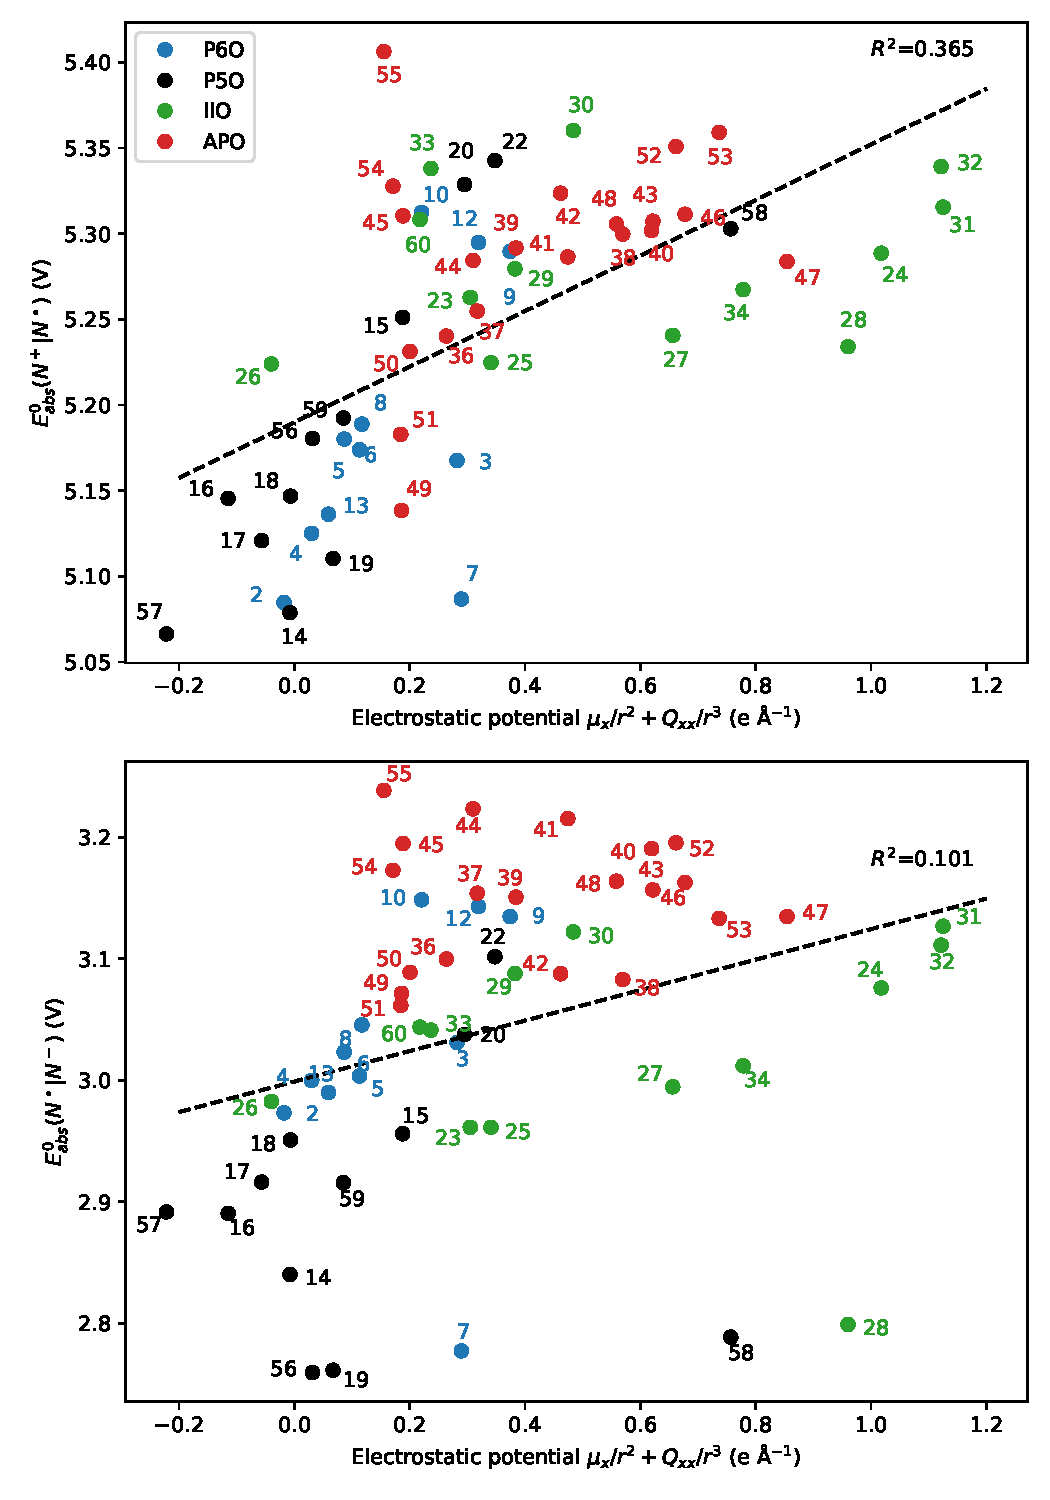
\includegraphics[width=\linewidth]{Figure6}
\caption{The different nitroxides considered in this work, sorted by families. Compounds \textbf{1}-\textbf{54} are from Ref.~\citenum{hodgsonOneElectronOxidationReduction2007}, while compounds \textbf{55}-\textbf{61} where considered for completeness. Experimental (reduction or oxidation) potentials are available in water if the number is written in red, while they are available in acetonitrile if the number is underlined.}
\label{fig:nitroxides}
\end{figure}

Geometry optimizations and subsequent vibrational frequency calculations were performed at the $\omega$B97X-D/6-311+G(d) level in water and acetonitrile (described using the SMD \cite{marenichUniversalSolvationModel2009} approach) with Gaussian 16 C02 \cite{g16}. For compound \textbf{1}-\textbf{54}, the geometries obtained by Hodgson et al. \cite{hodgsonOneElectronOxidationReduction2007} have been used as a starting point, taking advantage of their extensive conformational search. All radical forms are considered to have a doublet ground state. Then, the same calculations were preformed in acetonitrile for the subset of compounds for which experimental redox potentials are available (listed in Fig.~\ref{fig:nitroxides}). Finally, to study the influence of the substituent on the redox potential, following Zhang and co-workers \cite{zhangEffectHeteroatomFunctionality2018}, single point calculation are performed at the $\omega$B97X-D/6-311+G(d) level in gas phase, using the optimized geometries of  the radical states of each nitroxides (in water) in which $>$\ce{N-O^.} moiety is substituted by \ce{CH_2} (the rest of the geometry is kept fixed).

Since all thermochmical quantities are $\kappa$-dependent, analyses were performed thanks to the help of homemade Python scripts. When required [\textit{i.e.}, in Eq.~\eqref{eq:dh}], the value of $a$ (radius of the solute cavity) is taken as half the largest distance between two atoms in the molecule. Furthermore, a value of $\varepsilon_{r,wa}=80$ ($\varepsilon_{r,ac}=35$ ) is used for water (acetonitrile). These relative permitivities are the one of pure solvent, and are known to be lower in corresponding electrolytes \cite{silvaTrueHuckelEquation2022}. These variations can be, indeed, quite substantial (for example, $\varepsilon_r\approx 70$ for a solution containing \SI{1}{\mol\per\kilo\gram} of \ce{NaCl} in water \cite{kontogeorgisDebyeHuckelTheoryIts2018,silvaTrueHuckelEquation2022}), but depends on the nature of the electrolyte.
The value of $\kappa^2$ is obtained assuming  $c_{ox} = c_{rad} = c_ {red} = \SI{1e-3}{\mole\per\liter}$, a prototypical concentration in measurements.

\clearpage

\section{Results and discussion}

\begin{itemize}
	\item High-concentration limit: CIP (also, structure-activity relationship for CIP!, see Figs.~\ref{fig:Kx1} and \ref{fig:Kx2}) and Matsui.
	\item Comparison to experiment
\end{itemize}

\subsection{Structure-activity relationships}

Oxidation and reduction potentials of the nitroxide radicals in water, grouped by family, are plotted in Fig.~\ref{fig:family}. In comparison to \textbf{1}, changing the molecular structure or adding substituent generally increase both the oxidation and reduction potentials. Concerning the impact of the structure, 6-members ring compounds (P6O and APO)  display larger reduction potentials than their 5-members ring counterparts (P5O and  IIO), while adding one or two (IIO and APO) aromatic rings increase both the oxidation and reduction potential. 

\begin{figure}[!h]
	\centering
	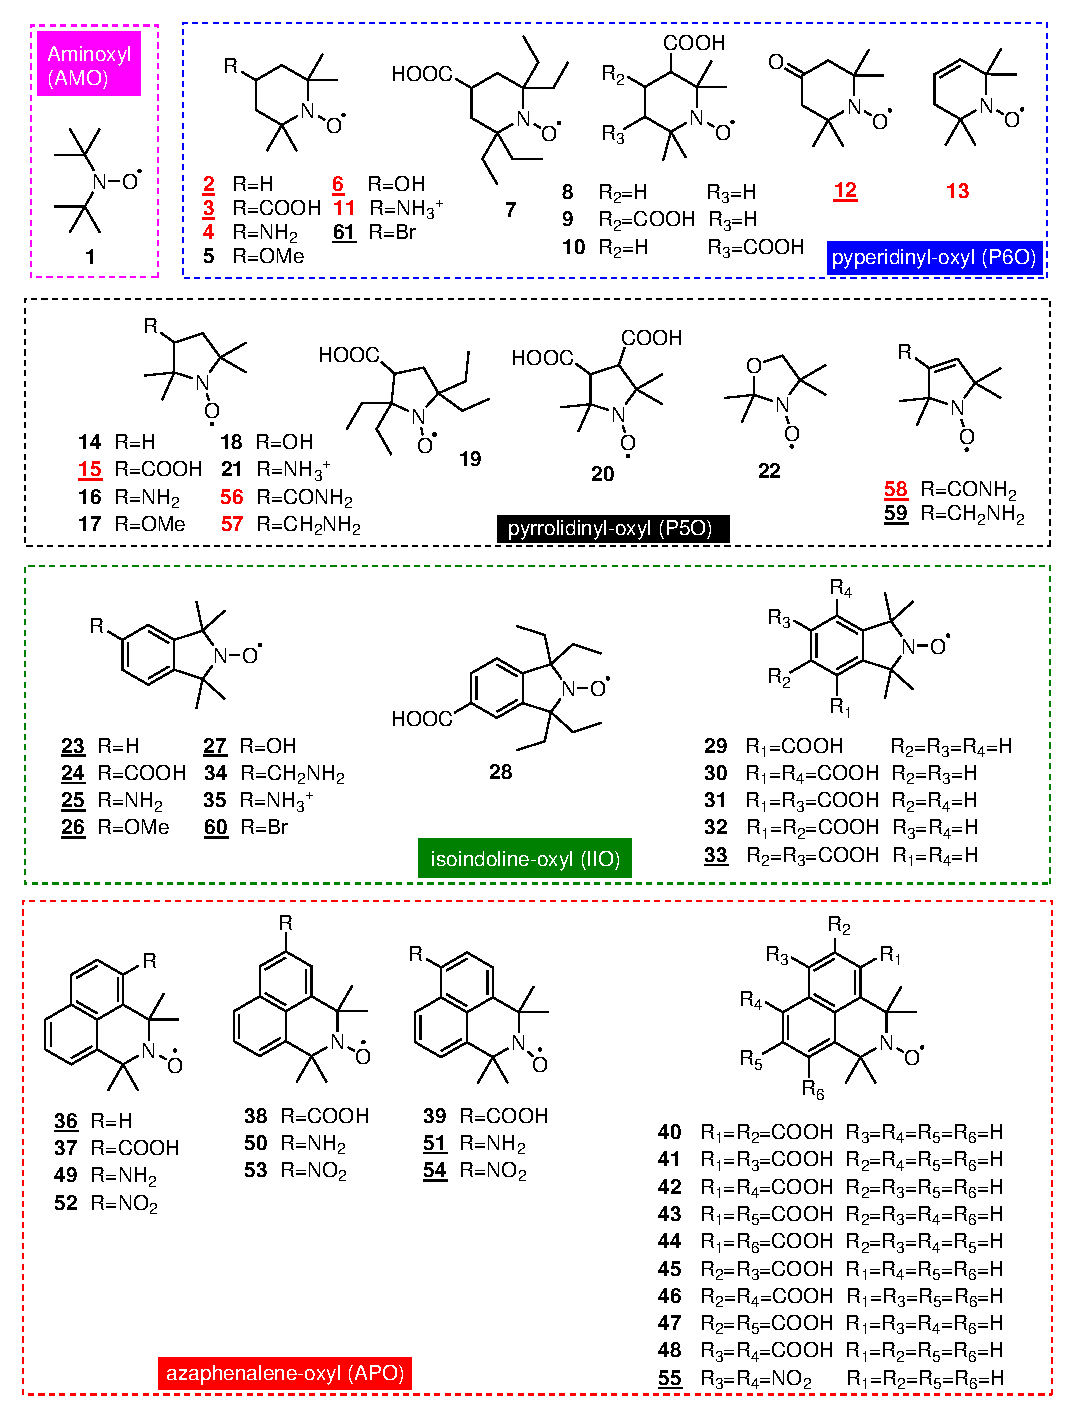
\includegraphics[width=.9\linewidth]{Figure7}
	\caption{Relationship between absolute oxidation and reduction potentials of nitroxides, as computed at the $\omega$B97X-D/6-311+G(d) level in water (SMD), with $[\ce{X}]=\SI{0}{\mole\per\liter}$. The color indicate the family (Fig.~\ref{fig:nitroxides}). For each of them, an ellipse is drawn, centered on the mean potential value among the family, and which width and height are given by the standard deviations.}
	\label{fig:family}
\end{figure}

Concerning the impact of the substituent, one can first notice than non-substituted nitroxides of each family (\textit{i.e.}, \textbf{2}, \textbf{14}, \textbf{23}, and \textbf{36}) have generally one of the lowest oxidation and reduction potential inside their group. Some trend also exists depending on the nature of the substituent: \begin{inparaenum}[(i)]
	\item shielding the radical center with ethyls instead of methyls (\textbf{7}, \textbf{19}, and \textbf{28}) results in a decrease of the potentials (especially the reduction), probably due to the change in inductive character, 
	\item  protonating \ce{NH2} increases the potentials, especially in P5O,
	\item multiple substitutions by COOH (\textit{e.g.},  \textbf{8} vs \textbf{9} and \textbf{10}) also increases the potentials, though less in IIO and APO, 
	\item mesomeric donors (\ce{NH2}, \ce{OH}, \ce{OMe}) substituted compounds have lower potentials than acceptor substituted ones (COOH, \ce{NO2}), especially in aromatic systems (IIO and APO), and
	\item  compound \textbf{56} and \textbf{58} have surprizingly low reduction potentials.
\end{inparaenum}
As a consequence, \textbf{55} have the largest oxidation and reduction potential of all the compounds studied in this paper.

To explain these effects, correlation of both potentials with Hammet constants have been attempted for P5O and P6O but turns out very weak, especially for the reduction (Fig.~S4).  The electrostatic interaction model [Eq.~\eqref{eq:Er}] provide more answers. Results are given in Fig.~\ref{fig:corr}. On the downside, this model fails to account for the effect of the substitution of methyls in ethyls.  Furthermore, including the disubstituted compounds (\textit{e.g.}, \textbf{9}) worsen the correlation ($R^2 \sim 0.5$ and 0.3 for oxidation and reduction, respectively); Finally, compounds \textbf{56} and \textbf{58} remain out of trend for reduction\todo{why?!?}. All  3 sets of compounds were thus treated as outliers. On the upside, it helps in explaining some the effect mentioned above: on the one hand, the increase in oxidation (and reduction) potential for aromatic compounds is correlated with an increase in quadrupole moment while, on the other hand, the modification due to donor/acceptor substituents are linked to change in the dipole moment. It also recover some of the effects due to the position of the substituent (see, \textit{e.g.} \textbf{49}-\textbf{51}), which was not  the case with the original model of Zhang and co-workers (resulting in weak correlations, $R^2\leq 0.3$).  Finally, while it is not applicable \textit{per se} to charged substituent (\textbf{11}, \textbf{21}, and \textbf{35}, for which the multipole moment are ill-defined), the leading term $q/r$ would result in a positive of $E_r$, well correlated with the increase in oxidation and reduction potential for these compounds. 

\begin{figure}[!h]
\centering
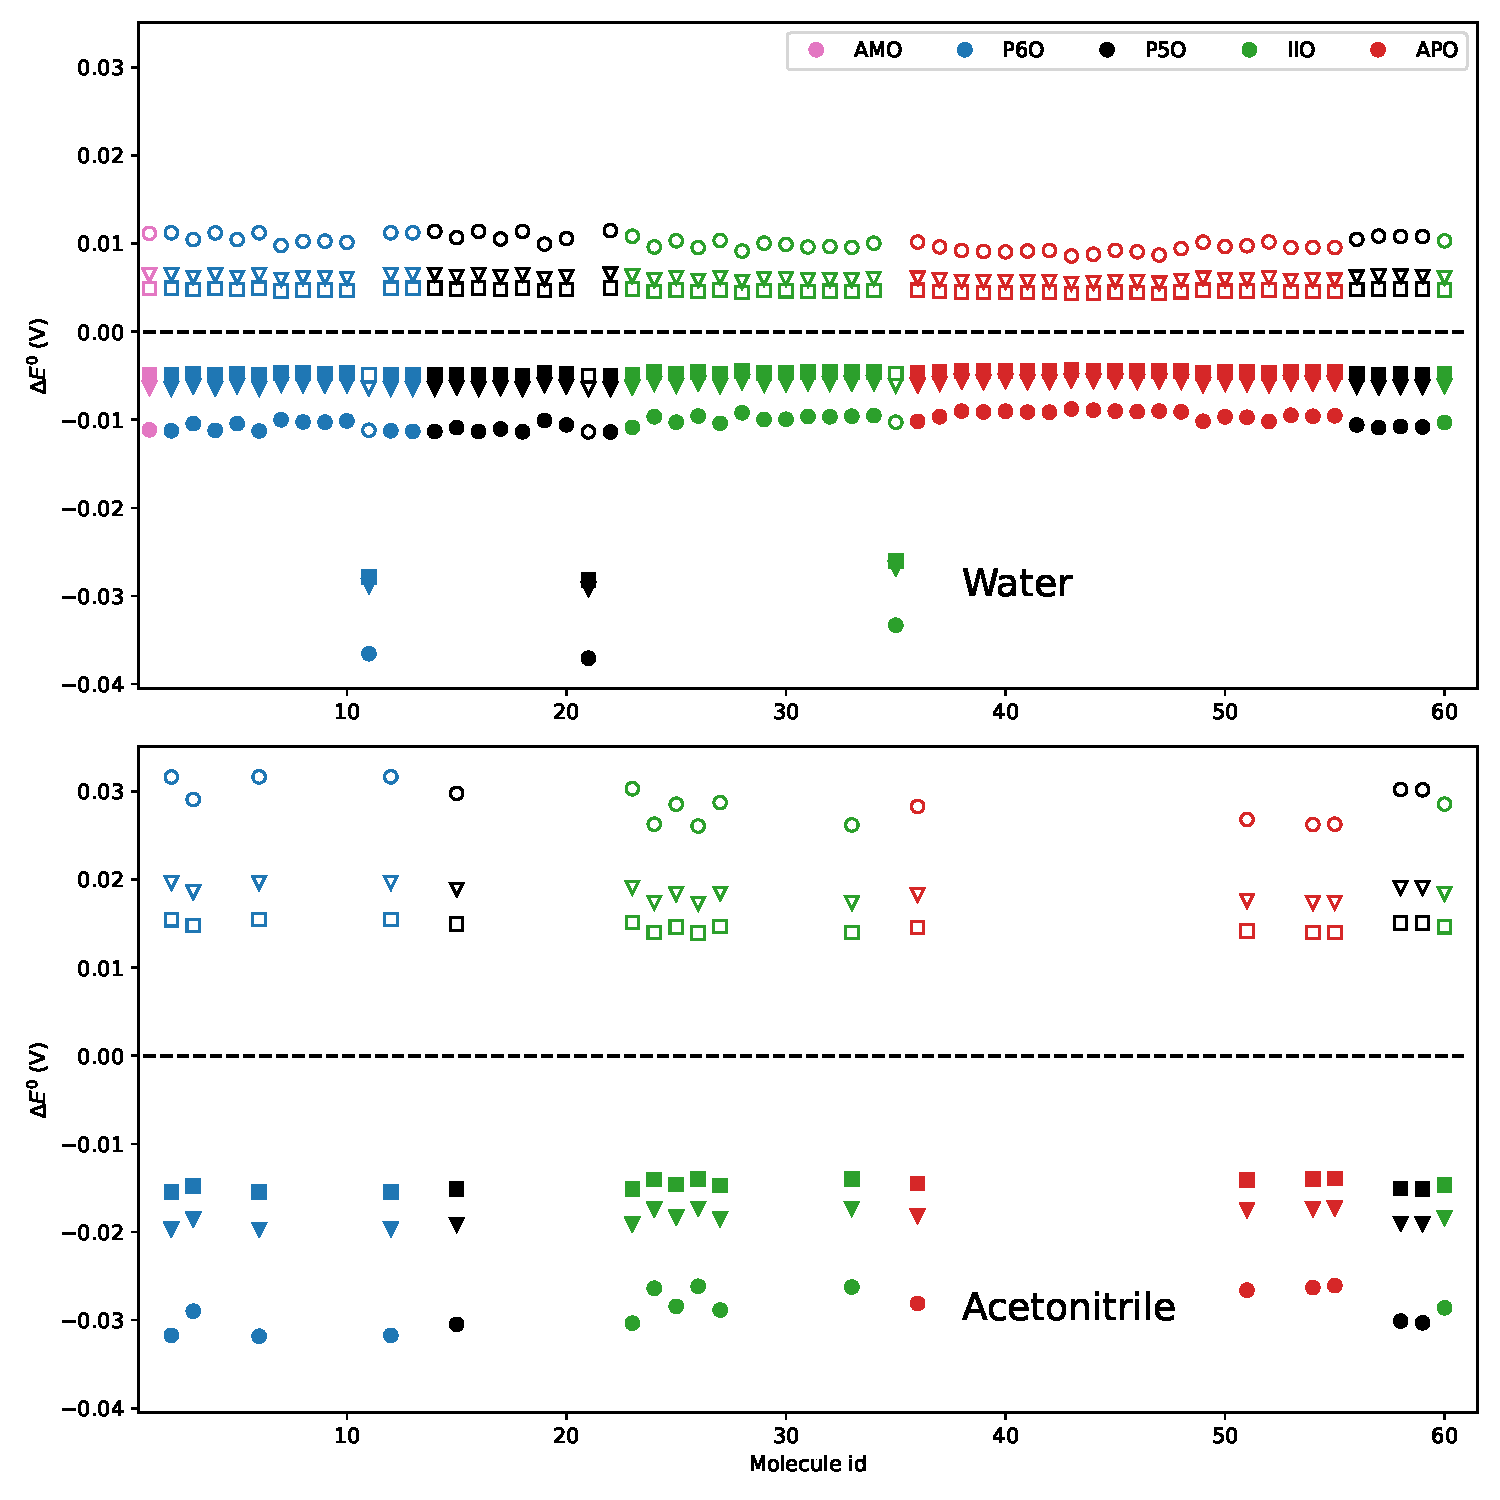
\includegraphics[width=\linewidth]{Figure8}
\caption{Relationship between absolute oxidation (top) and reduction (bottom) potentials of nitroxides and the electrostatic potential between the redox center ($>$\ce{N-O^.}) and the substituent, as computed at the $\omega$B97X-D/6-311+G(d) level in water (SMD), with $[\ce{X}]=\SI{0}{\mole\per\liter}$. Triangular marker ($\blacktriangle$) indicates results that are excluded from the correlation (see text).}
\label{fig:corr} 
\end{figure}

\clearpage

\subsection{Impact of the solvent}

The difference between redox potentials computed in water and acetonitrile is reported in Fig.~\ref{fig:watvsac}: except for compound \textbf{12}, the oxidation potential is only slightly affected, while there is a difference of $>$\SI{0.5}{\volt} for the reduction potentials. As a first approximation, the Born model [Eq.~\eqref{eq:born}] can explain these results: for the oxidation, the change in potentials in the two solvent, $E^0_{ac} - E^0_{wa}$, is proportional to $ \varepsilon_{r,ac}^{-1}-\varepsilon_{r,wa}^{-1}$, which is positive (assuming that \ce{N^.} is neutral, which is the case for the subset of compounds considered here), while for the reduction, it is proportional to $ \varepsilon_{r,wa}^{-1}-\varepsilon_{r,ac}^{-1}$, which is negative.  Since this impact is systematic, similar trends between redox potentials in water and acetonitrile are expected.

\begin{figure}[!h]
	\centering
	\includegraphics[width=\linewidth]{Figure9}
	\caption{Comparison between absolute oxidation (left) and reduction (right) potentials of nitroxides as computed at the $\omega$B97X-D/6-311+G(d) level in water and acetonitrile (SMD), with $[\ce{X}]=\SI{0}{\mole\per\liter}$. The dashed line represents no change. }
	\label{fig:watvsac}
\end{figure}

\subsection{Impact of the electrolytes}

So far, the concentration in electrolyte, $[X]$, was set to zero. To assess its impact on the redox potentials, the DH correction is first scrutinized in Fig.~\ref{fig:DH}. As expected, it is small in the range of concentration considered here (a few hundredth of \si{\volt} for $[X] \leq \SI{1}{\mole\per\liter}$ and larger in acetonitrile) and it increases with $[X]$. Its sign is different for oxidation and reduction potential. It is also smaller for compounds belonging to the IIO and APO family (being larger molecules with larger $a$), but larger for species with a net positive charge (\textbf{11}, \textbf{21}, \textbf{35}) for which the correction for oxidation and reduction are negative. 


\begin{figure}[!h]
	\centering
	\includegraphics[width=\linewidth]{Figure10}
	\caption{Impact of the Debye-Huckel correction, as $\Delta E^0 = -\frac{\Delta \Delta G_{DH}^\star}{F}$ for $[X]=\SI{1}{\mole\per\liter}$ (round markers), $[X]=\SI{0.1}{\mole\per\liter}$ (triangular markers, $\blacktriangle$)  and $[\ce{X}]=\SI{0}{\mole\per\liter}$ (square markers, $\blacksquare$), as computed at the $\omega$B97X-D/6-311+G(d) level in water (top) and acetonitrile (bottom) using SMD. Filled (empty) markers represent the correction to the oxidation (reduction) potential. }
	\label{fig:DH}
\end{figure}


\begin{figure}[!h]
\centering
\includegraphics[width=\linewidth]{Figure11}
\caption{Value of the complexation equilibrium constants $K_{01}$ (round markers, $\bullet$) and $K_{21}$ (square markers, $\blacksquare$), as computed at the $\omega$B97X-D/6-311+G(d) level in water (top) and acetonitrile (bottom) using SMD and $[X]=\SI{1}{\mole\per\liter}$.  The dashed line is there to help visualization. }
\label{fig:Kx1}
\end{figure}


\begin{figure}[!h]
\centering
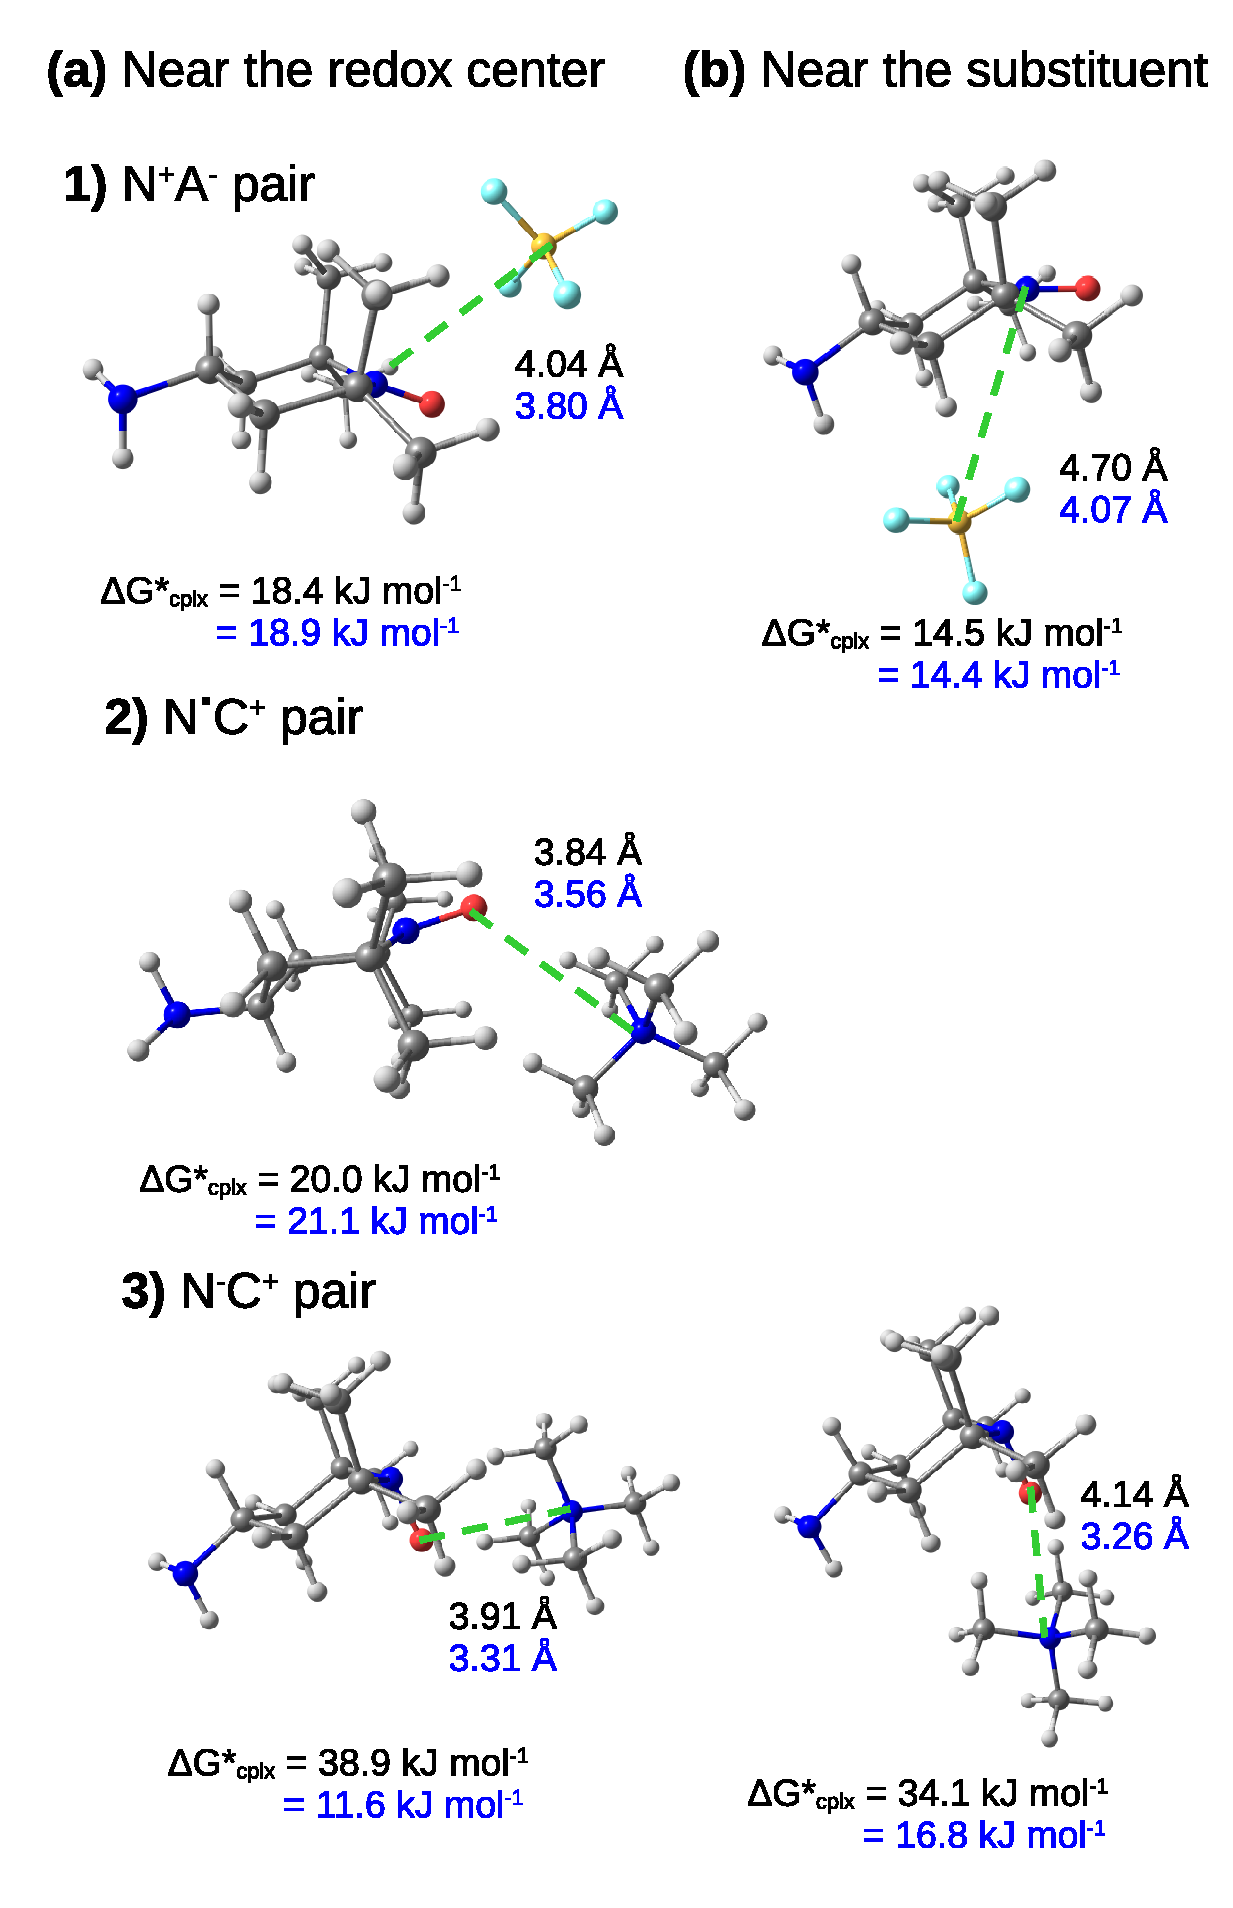
\includegraphics[width=\linewidth]{Figure12}
\caption{Value of the complexation equilibrium constants $K_{02}$ (round markers, $\bullet$), $K_{12}$ (triangular markers, $\blacktriangle$) and $K_{22}$ (square markers, $\blacksquare$) for the 3 oxidation state of nitroxides, as computed at the $\omega$B97X-D/6-311+G(d) level in water (top) and acetonitrile (bottom) using SMD and $[X]=\SI{1}{\mole\per\liter}$.  The dashed line is there to help visualization. }
\label{fig:Kx2}
\end{figure}

\clearpage
\section{Conclusion}

Well.
	
	
\bibliographystyle{elsarticle-num-names} 
\bibliography{biblio}
	
\end{document}
\endinput
%%
%% End of file `elsarticle-template-num.tex'.
